\section{Introduction}\label{sec:intro}

\subsection{Problem Background}

The carbon cycle describes the process of the exchange of carbon throughout the geochemical cycle of the Earth, and is a vital component for life on the planet. One key component of this part of the process is the decomposition of plant material and woody fibers. Some of the key agents in decomposing woody fibers are fungi. This problem requires the model for the the decomposition ability of fungi community.

\subsection{Problem Restatement}
\begin{itemize}
    \item Describes the breakdown of ground litter and woody fibers through fungal activity in the presence of multiple species of fungi.
    \item Incorporate the interactions between different species of fungi, which have different growth rates and different moisture tolerances.
    \item Analyze model and describe the interactions between the different types of fungi, for both short and long term trends.
    \item Examine the sensitivity to rapid fluctuations in the environment and determine the overall impact of changing atmospheric trends.
    \item Include predictions about the relative advantages and disadvantages for each species and combinations of species likely to persist, and do so for different environments including arid, semi-arid, temperate, arboreal, and tropical rain forests.
    \item Describe how the biodiversity impacts the overall efficiency with respect to the breakdown of ground litter. Predict the importance and role of biodiversity in the presence of different degrees of variability in the local environment.
\end{itemize}


\subsection{Our Work}

We separated the problem into several parts, do modeling, the combined them together as shown in figure \ref{fig:workflow}.

\begin{figure}[ht]
    \caption{Work flow of our modelling}\label{fig:workflow}
    \begin{center}
        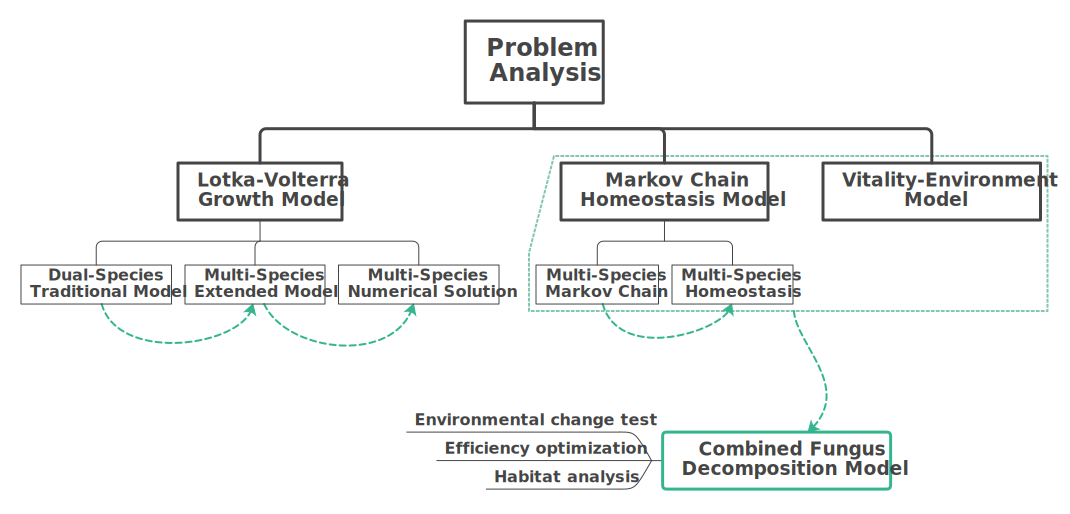
\includegraphics[width=\columnwidth]{workflow.pdf}
    \end{center}\end{figure}
